\section{Séquençage nouvelle génération}
\subsection*{Historique}
	Le séquençage de l'ADN a été inventé dans la fin des années 1970.
Deux méthodes ont été développées indépendamment.
L'une, basé sur la \textbf{synthèse enzymatique} sélective et réalisé par l'équipe de Frederick Sanger en Angleterre.
La deuxième, basé sur la \textbf{dégradation chimique} sélective a été réalisée par l'équipe de Walter Gilbert aux États-Unis.
Tout deux ont été récompensé du prix Nobel de chimie pour cette découverte en 1980.\\


La technique de séquençage de Walter Gilbert était le prémisse du pyroséquençage. Cette technique est principalement basé sur l'addition d'un seul nucléotide qui est révélé en temps réel par détection de la  luminescence. 
~~\\
Au début du XXème siècle, de nouvelles techniques de séquençage couplées aux connaissances en physique, chimie, informatique, nanotechnologie et biotechnologie ont vu le jour, et permettent d'augmenter le débit du séquençage par une parallélisation massive des réactions et par miniaturisation des supports utilisés.
~~\\
Nous allons décrire deux plateformes de séquençage novatrices qui, aujourd'hui encore, sont les modèles en matière de séquençage haut-débit :
~~\\
\begin{itemize}
\item[$\bullet$]la technologie 454 (le pyroséquençage),
\item[$\bullet$]la technologie Solexa (Illumina).
\end{itemize}
	
\subsection*{Les différents types de séquençage haut-débit{\scriptsize \cite{NGS}\cite{NGS2}\cite{NGS3}\cite{NGS4}\cite{NGS5}}}
	\subsubsection*{Le pyroséquençage}

Le pyroséquençage est donc une version améliorée de la technique de Maxam et Walter. Il a été élaboré par Hyman et al., un groupe suédois. Le principe est d'utiliser la technique de Walter en l'a couplant avec la technique de PCR (Réaction en Chaine par Polymerase). C'est une technique de séquençage par \textbf{synthèse}.

~~\\
Premièrement, on réalise une bibliothèque des séquences que l'on veut séquencé (à l'aide d'une séquence de ligation qui va se coupler à la séquence).

~~\\
On extrait la séquence puis on lui fixe une séquence dite adapteur. La séquence adapteur est complémentaire d'une séquence fixée à une micro-bille. On attache donc la séquence d’intérêt à une micro-bille. On dispose de nombreuses micro-billes préparées de la même façon dans des puces à ADN puis on polymérise la séquence par PCR (Fig. 1 et 2).
\newpage
\begin{figure}[!h]
 \centering
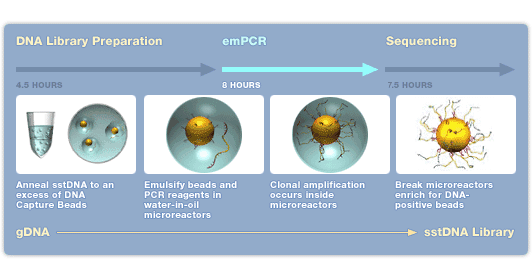
\includegraphics[scale=0.8]{Images/microbille.png}
\caption{Ligation des séquences aux microbilles.}
\end{figure}

\begin{figure}[!h]
 \centering
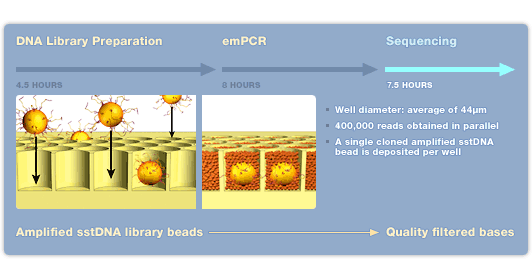
\includegraphics[scale=0.8]{Images/incbil.png}
\caption{Incorporation des billes dans la puce à ADN.}
\end{figure}

On dispose la puce dans une cuve contenant :
~~\\
\begin{itemize}
\item de la Sulfurylase,
\item de la Luciferase,
\item de l'Apyrase,
\item de la Polymerase.
\end{itemize}
~~\\
Le tableau ci-dessous explique le rôle de chacune des enzymes listées précédemment:
~~\\

\begin{tabular}{|c|c|c|c|c|}
	\hline
   Enzymes & Rôles \\
   \hline
   Sulfurylase & Convertie un pyrophosphate en adenosine tri-phosphate (ATP). \\
   \hline
   Luciferase & Emet de la lumière en consommant un ATP. \\
   \hline
   Apyrase & Dégrade les nucléotides. \\
   \hline
   Polymerase & Incorpore un acide nucléique complémentaire à un brin d'ADN \\&en consommant un groupement phosphate d'un ATP.\\
   \hline
\end{tabular}

~~\\
~~\\
Ensuite, on incorpore successivement les acides nucléiques de manière sélective au niveau de la puce.

A chaque incorporation d'acides nucléiques, le résidu attendu par la polymérase est intégré dans la chaine ADN pendant l'élongation et libère un pyrophosphate.

L’ATPsulfurylase vient alors transformer ce Pyrophophate (PPi) en ATP qui est alors utilisé, couplé à une Luciférine, par une Luciférase. On a alors production d’Oxyluciférine et d’un signal lumineux.

L'Apyrase dégrade les acides nucléotidiques en surplus dans le milieu (Fig. 3).
\begin{figure}[!h]
   \begin{minipage}[b]{0.40\linewidth}
      \centering 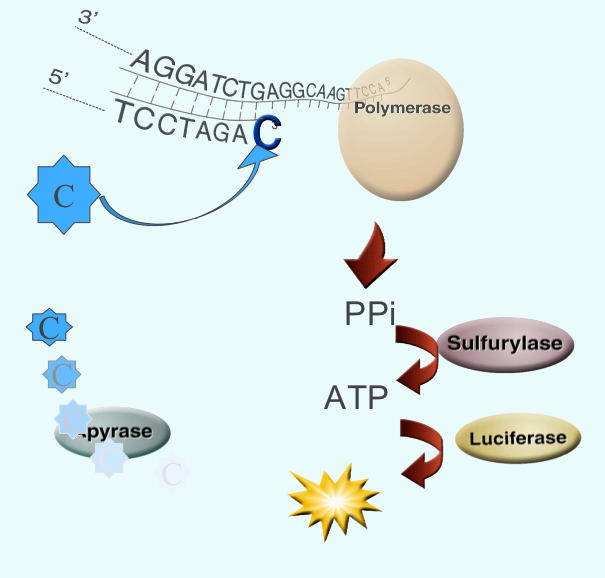
\includegraphics[scale=0.3]{Images/proces.png}
   \end{minipage}\hfill
   \begin{minipage}[b]{0.48\linewidth}   
      \centering 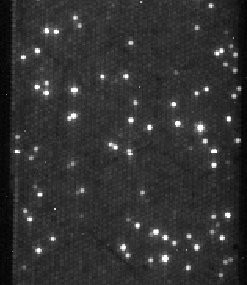
\includegraphics[scale=0.4]{Images/454.png}
   \end{minipage}
   \caption{Représentation des étapes réactionnelles pour obtenir le signal lumineux.}
\end{figure}
~~\\
Le signale lumineux est capté par un capteur CCD (Charge-Coupled Device) puis reproduit sous forme d’un pic sur le Pyrogramme.La hauteur de ce pic est fonction de l'intensité de la lumière, elle-même proportionnelle de la quantité de l'acide nucléique intégré (Fig. 4).
\begin{figure}[!h]
   \begin{minipage}[b]{0.40\linewidth}
      \centering 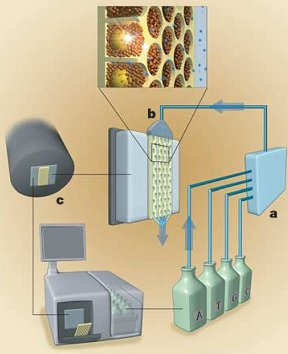
\includegraphics[scale=0.5]{Images/mach.png}
   \end{minipage}\hfill
   \begin{minipage}[b]{0.48\linewidth}   
      \centering 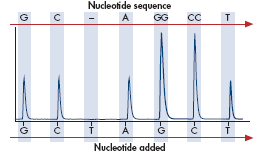
\includegraphics[scale=0.7]{Images/sign.png}
   \end{minipage}
   \caption{Lecture de la séquence à partir des signaux lumineux.}
\end{figure}
\paragraph*{Technique de séquençage Illumina}

Illumina est le nom d'un laboratoire développant entre autre le séquençage à partir de la technique de Sanger (la CRT: Cyclic Reversible Termination) ainsi que des connaissances actuelles en biopuces à ADN, nanotechnologies et en informatique de pointe pour l'acquisition, le traitement et l'analyse des images.
~~\\
Cette technique s'applique en plusieurs étapes :
~~\\
\textbf{Étape 1:}
Préparation de la banque d'ADN génomique.
L'ADN génomique est fragmenté par nébulisation. Les extrémités sont réparées et des adaptateurs sont fixés sur chaque extrémité par ligation.
~~\\
\textbf{Étape 2:}
Des ponts d'amplification sont formés sur des plaques ce qui permet d'obtenir de grandes quantités de brins d'ADN, augmentant ainsi le débit de séquençage.
~~\\
\textbf{Étape 3:}
Les brins sont ensuite dénaturés et l'on effectue le séquençage par la technique CRT. 
Les nucléotides fluorescents sont additionnés d'un groupement nitrophenyl en 3'O.
Le nucléotide est incorporé à la séquence lors de la synthèse.
Ensuite, il y a une phase de détection du nucléotide inséré par fluorescence.
L'envoi d'un rayonnement UV (>300nm) détache le groupement nitrophenil de la liaison en 3'O permettant l'incorporation de nouveaux nucléotides.
~~\\
\textbf{Étape 4:}
Interprétation des résultats et lecture de la séquence (Fig. 5).
\begin{figure}[!h]
 \centering
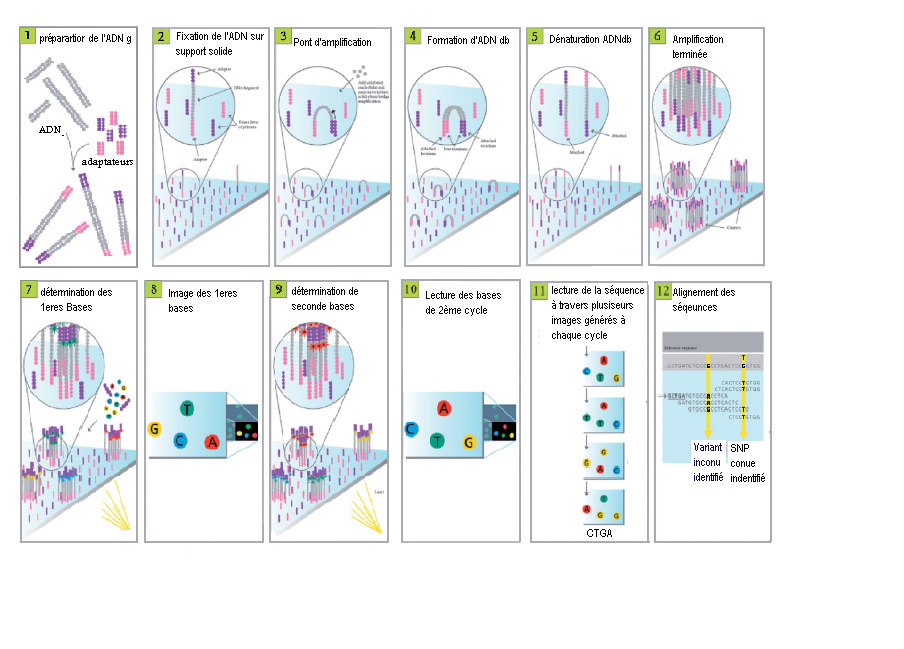
\includegraphics[scale=0.6]{Images/sequfr1.png}
\caption{Différentes étapes de la méthode de séquençage Illumina.}
\end{figure}
~~\\